\chapter{Opis projektnog zadatka}

			Sinappsa je web aplikacija koja omogućuje studentima FER-a da traže ili pružaju pomoć oko specifičnog gradiva, laboratorijskih vježbi ili kolegija općenito. Student-pomagač će moći staviti oglas na koji će se drugi studenti moći javljati. Nakon obavljenih instrukcija student daje recenziju studentu-pomagaču. Ta recenzija ulazi u cjelokupni rejting studenta koji se zatim prikazuje na rejting listi na web stranici. Prikaz rejting liste sadrži 10 registriranih članova s najvećim rejtingom i ažurira se redovito.
			
			Aplikacija se sastoji od tri vrste korisnika, a to su:
			\begin{packed_enum}
				\item neregistrirani korisnici
				\item registrirani korisnici 
				\item moderatori
			\end{packed_enum}
		
	\noindent \textbf{Neregistrirani korisnici}
	
			Neregistrirani korisnici na stranici vide objavljene oglase i rejting listu pod korisničkim imenom. Mogu filtrirati oglase po smjeru, kolegiju i kategoriji. Za smjer, padajući izbornik daje opcije elektrotehnika, računarstvo i nerazvrstani, a za kategoriju su moguće opcije laboratorijska vježba, blic, gradivo, kontinuirani ispit i ispitni rok.
			
			Ovim korisnicima nije dopušteno javljanje na oglase koje vide već se za tu mogućnost moraju registrirati službenom FER e-mail adresom. Opcija registracije ili prijave pojavljuje im se u padajućem izborniku klikom miša na ikonu u gornjem desnom kutu. Odabirom jedne od opcija, odlazi se na formu za registraciju ili prijavu.
			
			Već prije registrirani korisnik ima mogućnost prijave na svoj račun preko nadimka. Ako korisnik koji još nema račun završi na formi za prijavu, klikom na gumb „Nemaš račun?“ korisnik se preusmjerava na formu za registraciju. 
			
			Na formi za registraciju korisnik treba unijeti svoje ime, prezime, korisničko ime, avatara, e-mail i lozinku. Sustav provjerava pripada li e-mail adresa FER domeni. Nakon zahtjeva za registraciju, korisnik klikom na link u primljenom e-mail potvrđuje svoju registraciju.
			
			\begin{figure}[H]
				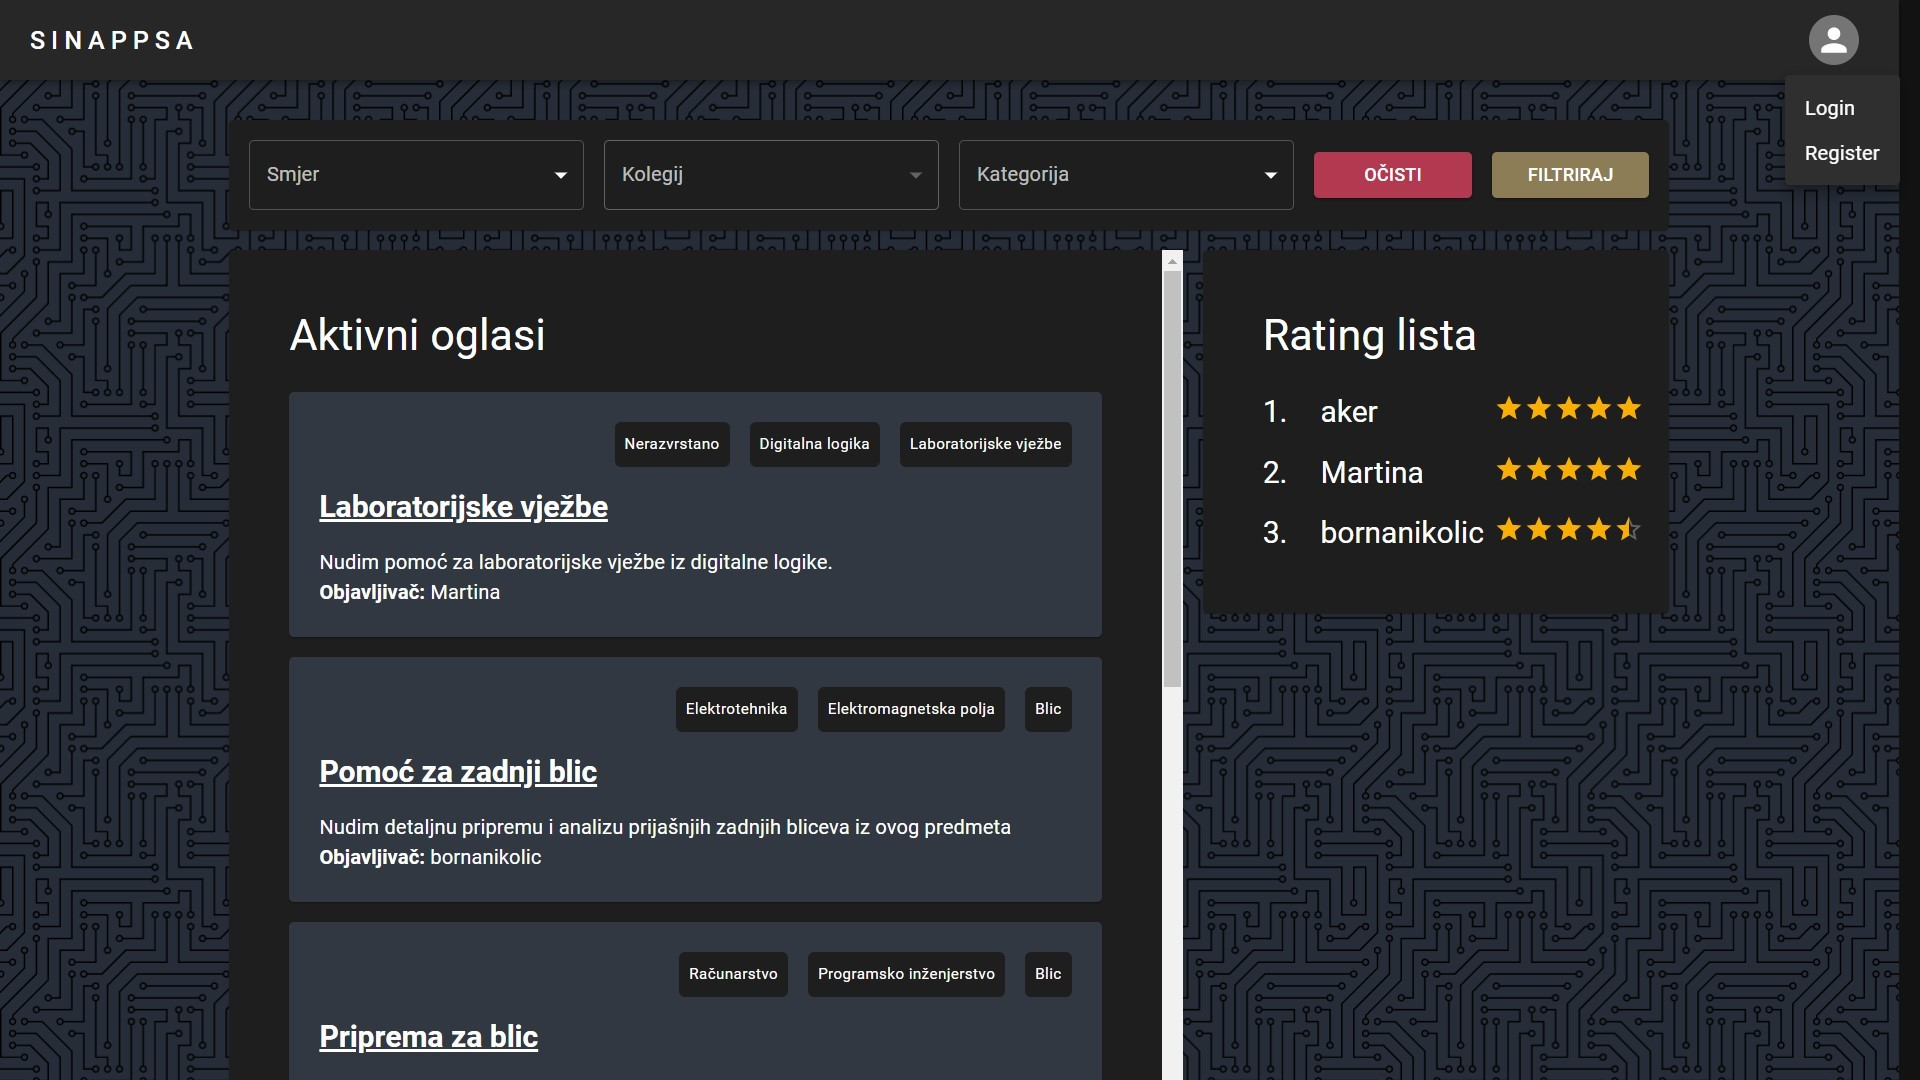
\includegraphics[scale=0.37]{slike/neregistrirani.jpg}
				\centering
				\caption{Početna stranica za neregistriranog korisnika}
				\label{fig:neregistriran}
			\end{figure} 
		
			\begin{figure}[H]
				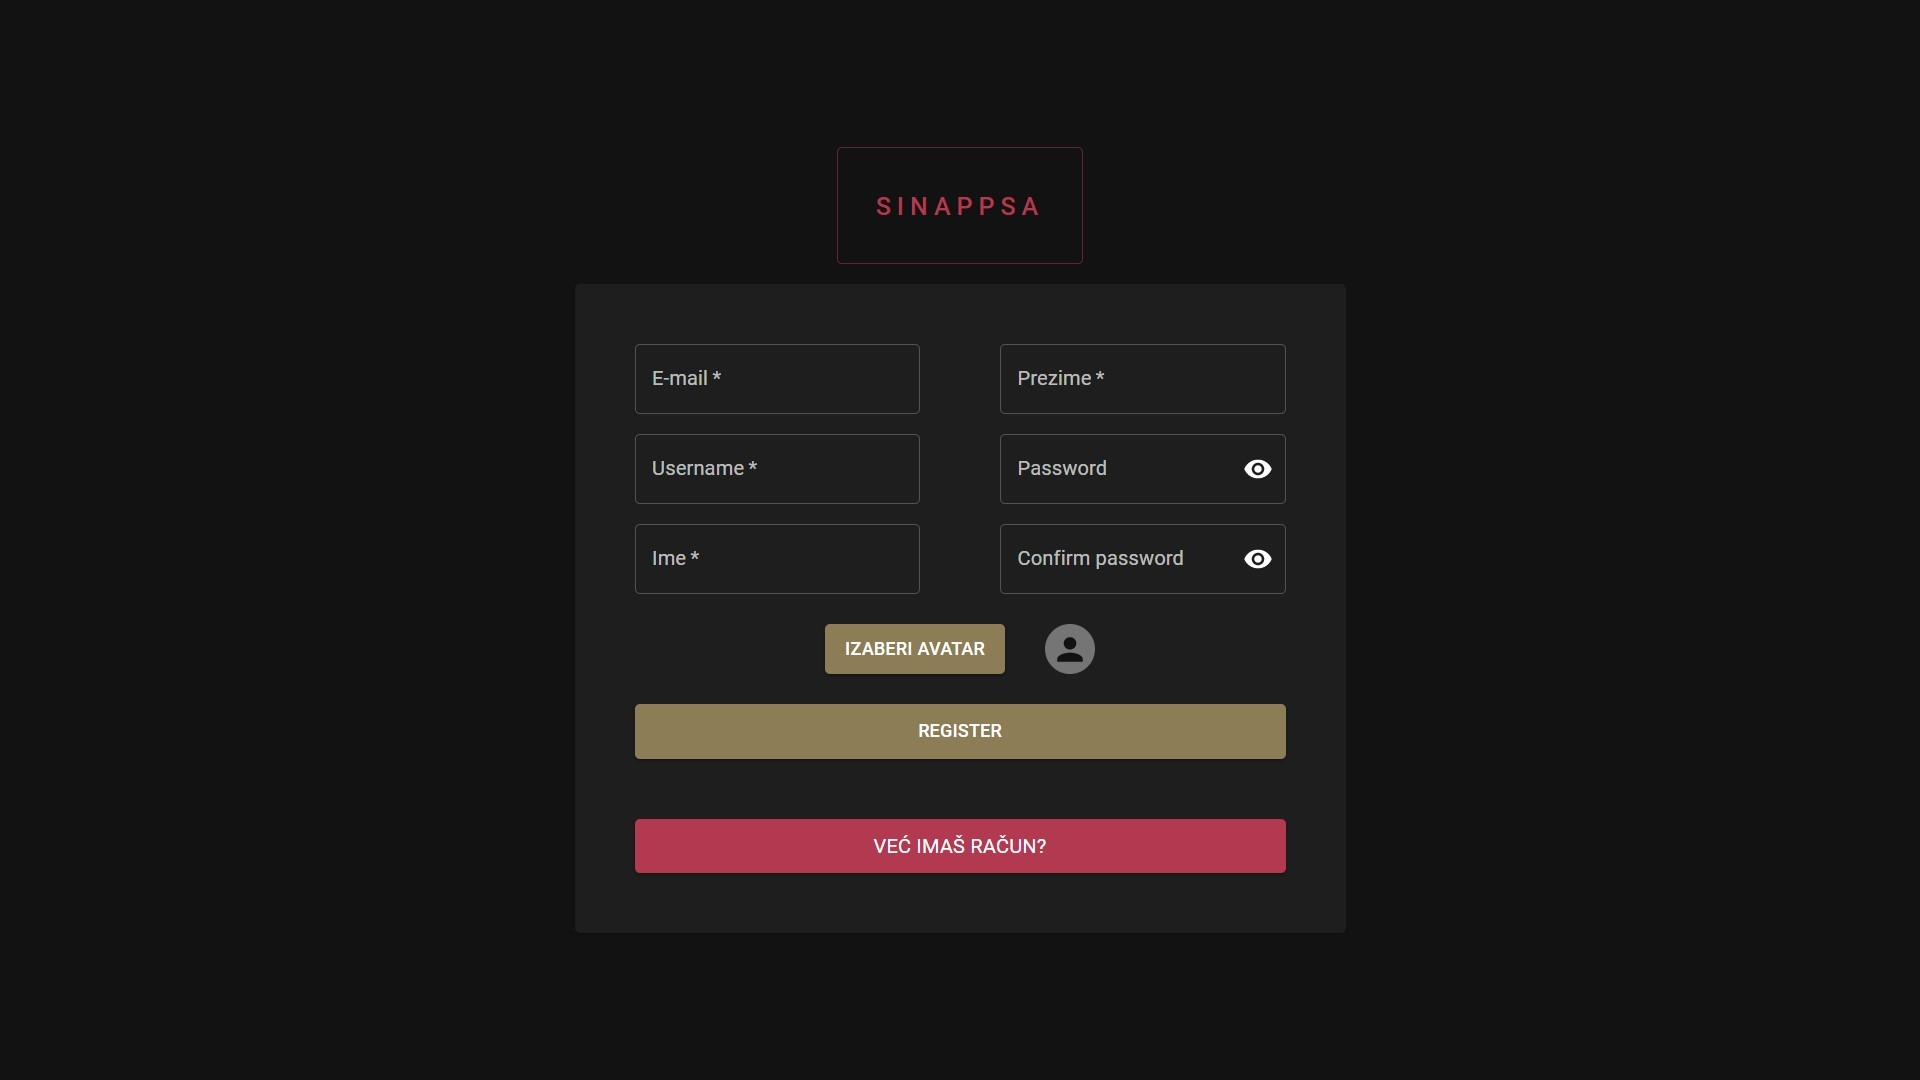
\includegraphics[scale=0.37]{slike/registracija.jpg} 
				\centering
				\caption{Forma za registraciju}
				\label{fig:registracija}
			\end{figure}
		
			\begin{figure}[H]
				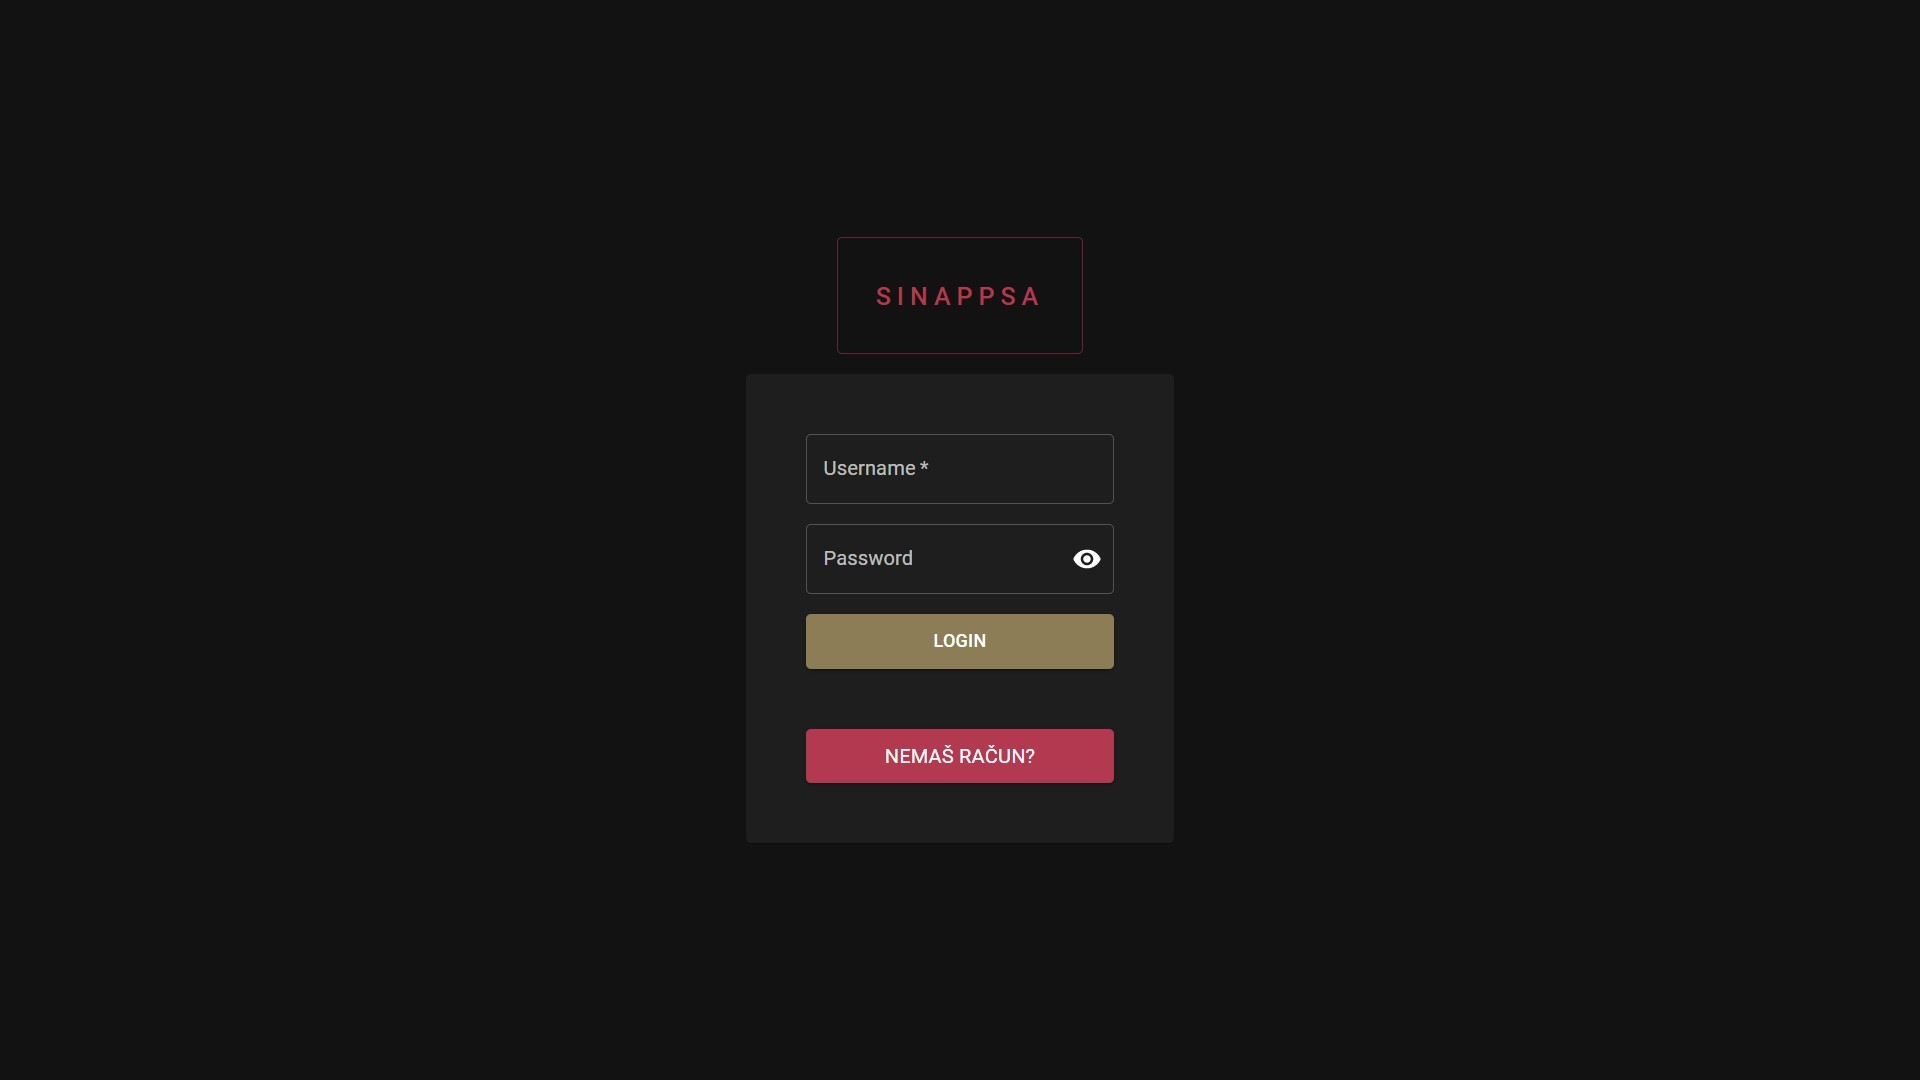
\includegraphics[scale=0.37]{slike/login.jpg} 
				\centering
				\caption{Forma za prijavu}
				\label{fig:prijava}
			\end{figure}
		
	\noindent \textbf{Registrirani korisnici}
	
			Registrirani korisnici, uz funkcionalnost neregistriranih korisnika, mogu objavljivati oglase i odgovarati na njih. Opcija stvaranja oglasa pojavljuje se u zaglavlju kao gumb „Dodaj oglas“. Pri stvaranju oglasa korisnik navodi naslov, opis, kolegij i kategoriju oglasa.
			
			Registrirani korisnici također mogu i odgovarati na oglase. Prilikom odgovora na oglas unosi se proizvoljna poruka koja se zajedno s kontakt informacijama korisnika šalje na e-mail adresu studentu-pomagaču. Daljnja komunikacija obavlja se preko e-maila. Upit na oglas može biti prihvaćen, odbijen ili u tijeku. Ako je korisnik dobio pozitivan odgovor, nakon odslušanih instrukcija, osoba ocjenjuje iste  te se ta ocjena pribraja u cjelokupni rejting studenta-pomagača. 
			
			\begin{figure}[H]
				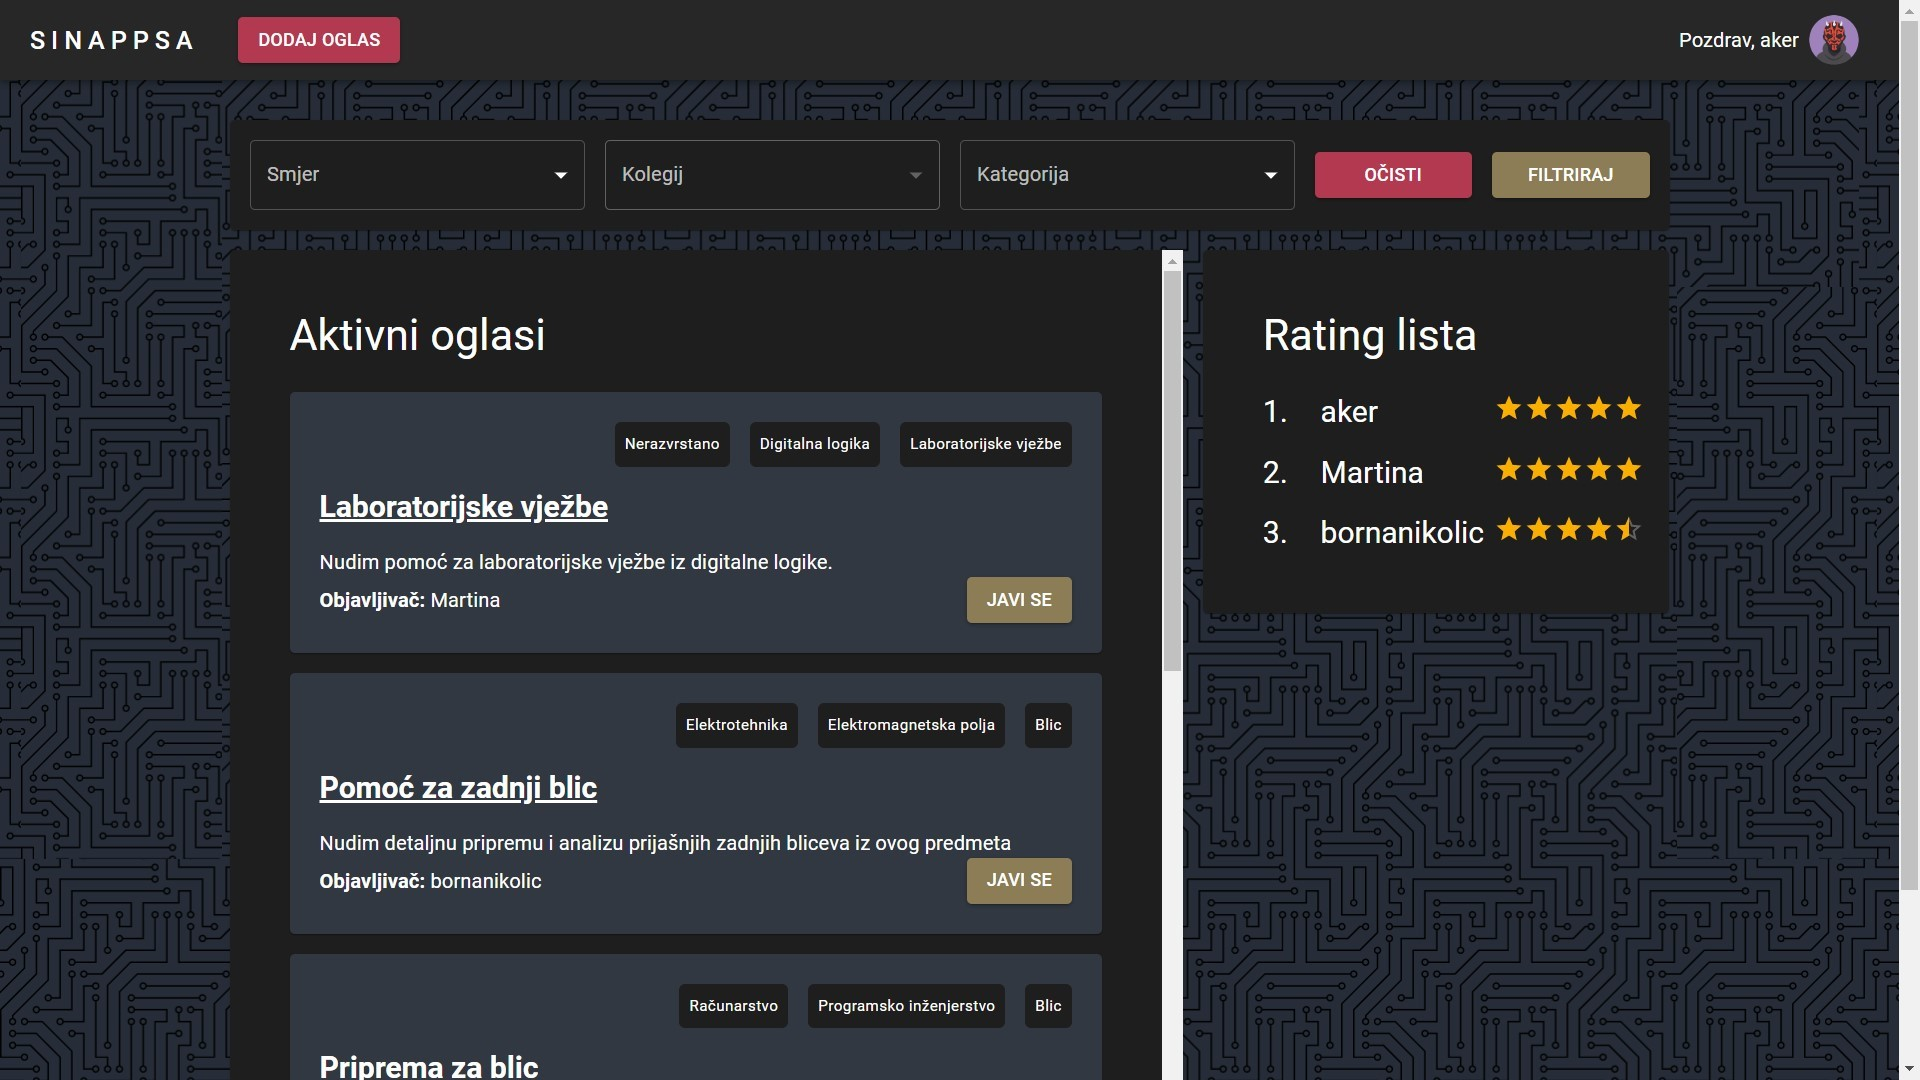
\includegraphics[scale=0.37]{slike/registrirani.jpg} 
				\centering
				\caption{Početna stranica za registriranog korisnika}
				\label{fig:registrirani}
			\end{figure}
		
			\begin{figure}[H]
				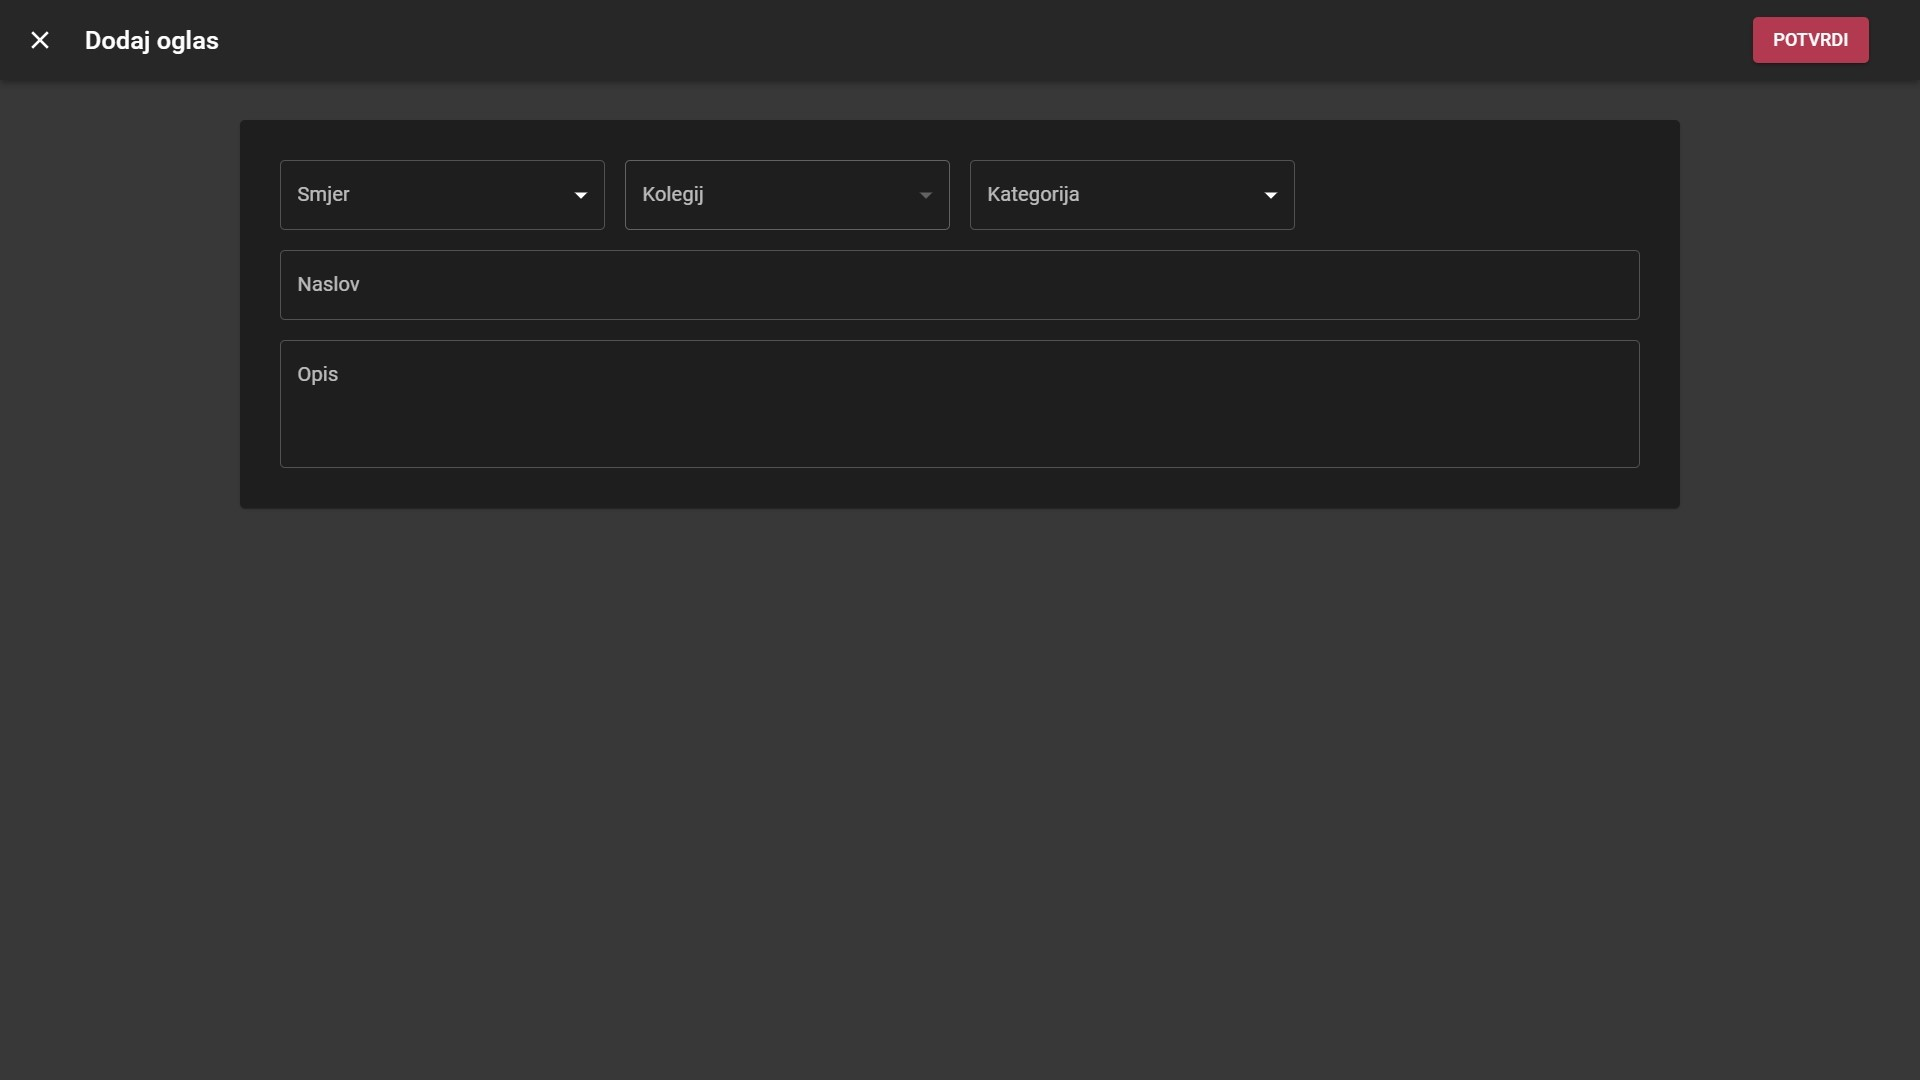
\includegraphics[scale=0.37]{slike/dodajOglas.jpg} 
				\centering
				\caption{Forma za dodavanje oglasa}
				\label{fig:oglas}
			\end{figure}
		
			Na svom profilu, korisniku se prikazuju njegovi aktivni oglasi, upiti na njegove oglase kao i statusi upita koje je korisnik poslao na druge oglase. Aktivnim oglasima može mijenjati naslov i opis te je u mogućnosti obrisati ih. Uz informacije o oglasima na profilu se nalaze i osobne informacije korisnika. Korisniku je omogućeno naknadno mijenjanje lozinke, korisničkog imena i avatara.
			
			\begin{figure}[H]
				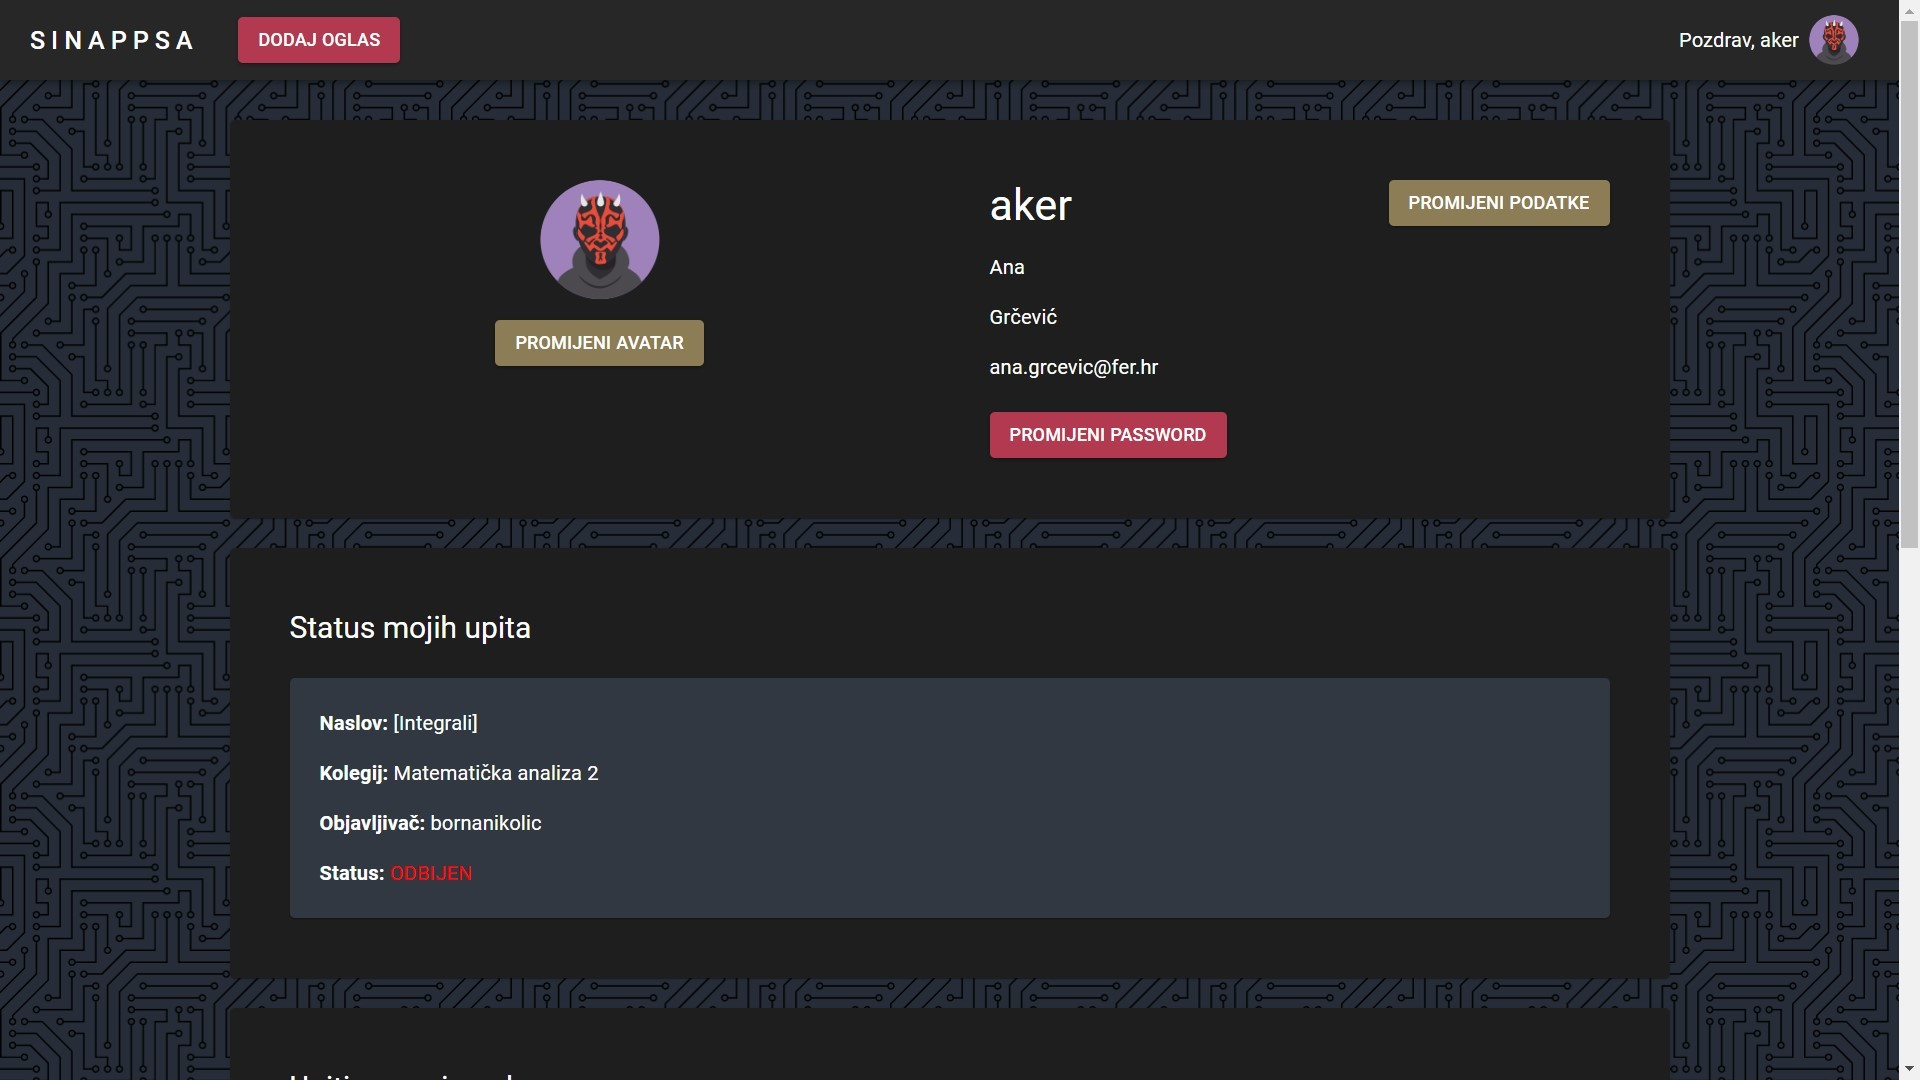
\includegraphics[scale=0.37]{slike/profil1.jpg} 
				\centering
				\caption{Izgled profila - prvi dio}
				\label{fig:profil1}
			\end{figure}
		
			\begin{figure}[H]
				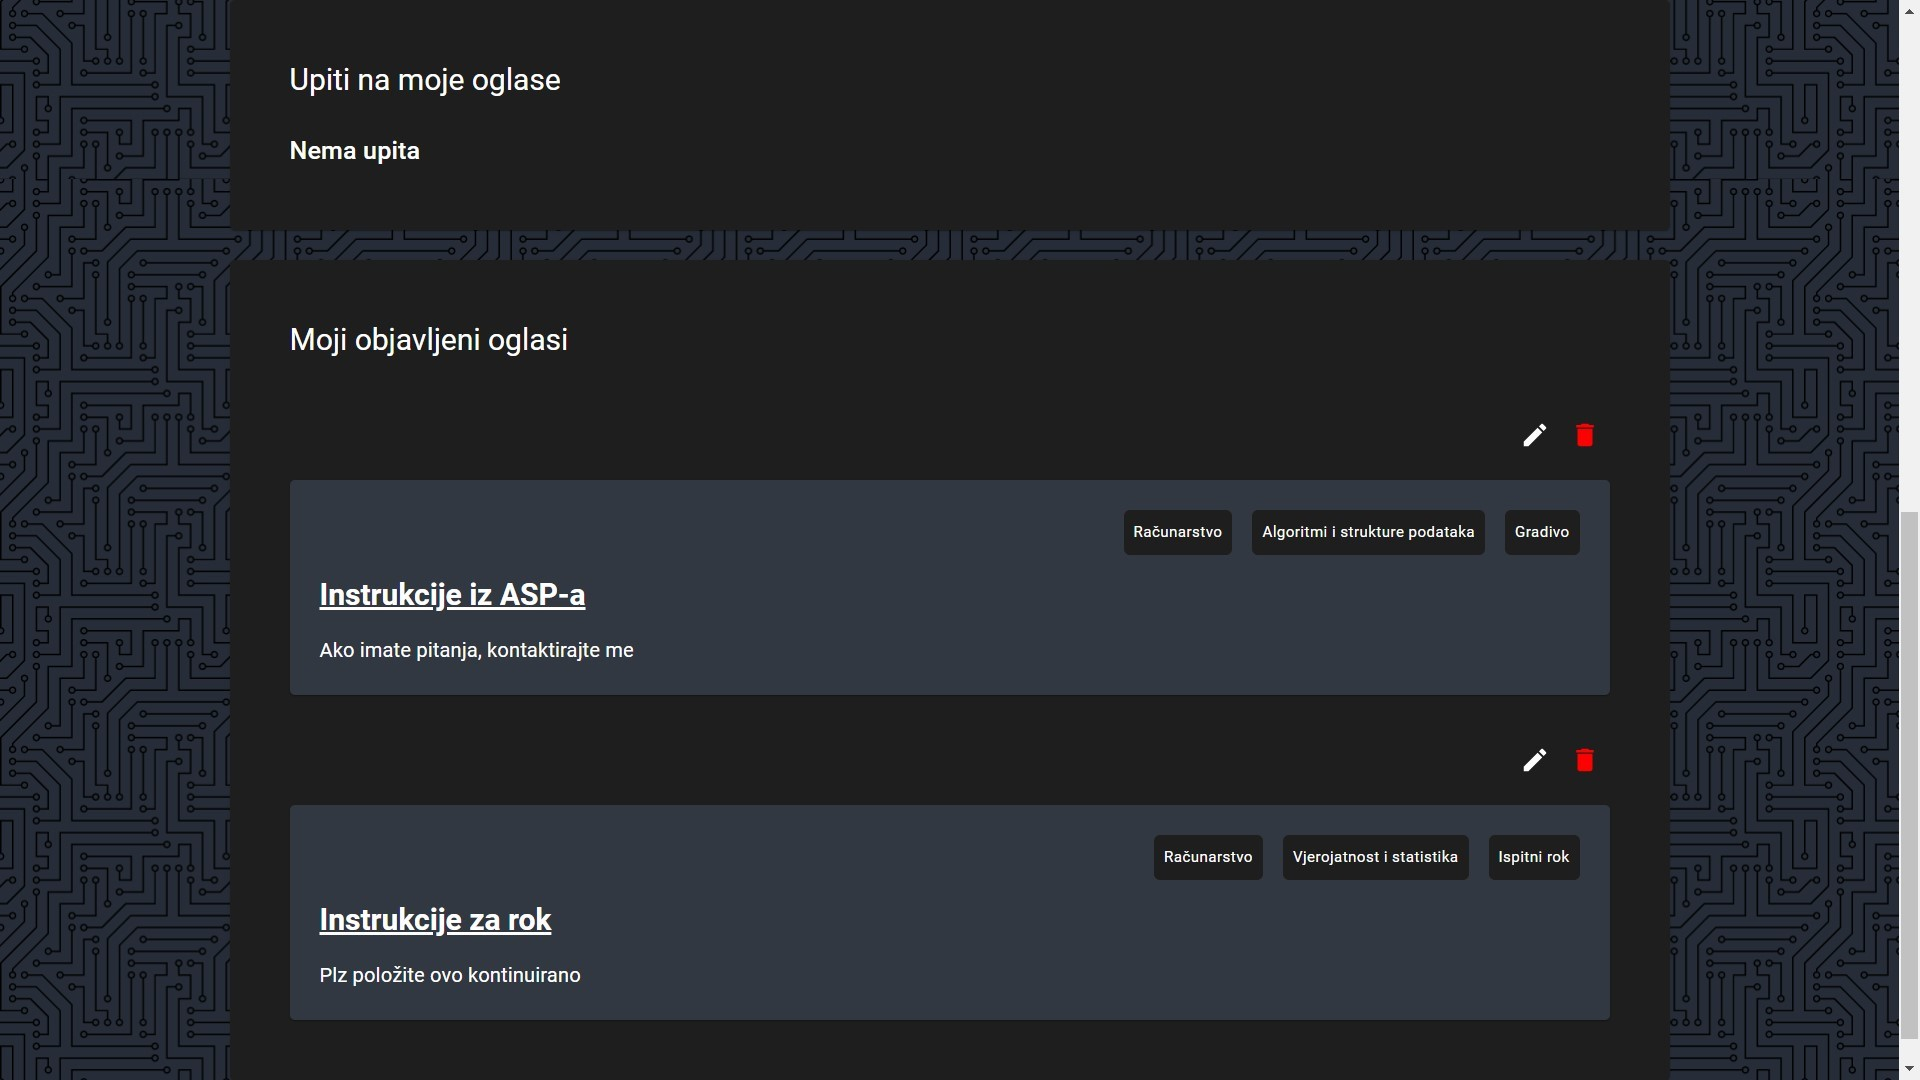
\includegraphics[scale=0.37]{slike/profil2.jpg} 
				\centering
				\caption{Izgled profila - drugi dio}
				\label{fig:profil2}
			\end{figure}
		
	\noindent \textbf{Moderator}
	
			Moderator ima ulogu uklanjanja nepravilnih ili neprikladnih oglasa. Kada moderator odabere opciju brisanja oglasa pojavljuje se skočni prozor u koji upisuje razlog zašto je oglas obrisan te se isti šalje na e-mail adresu objavljivaču oglasa. 
			
			Moderator također ima opciju dodavanja kolegija. Nakon odabira opcije „Dodaj kolegij“ koja se nalazi u zaglavlju, moderatoru se otvara skočni prozor gdje upisuje naziv kolegija koji želi dodati. Pored opcije "Dodaj kolegij" nalazi se gumb "Lista kolegija" čijim pritiskom se moderatoru prikazuje popis postojećih kolegija koje može uređivati, obrisati ili pretraživati.
			
			\begin{figure}[H]
				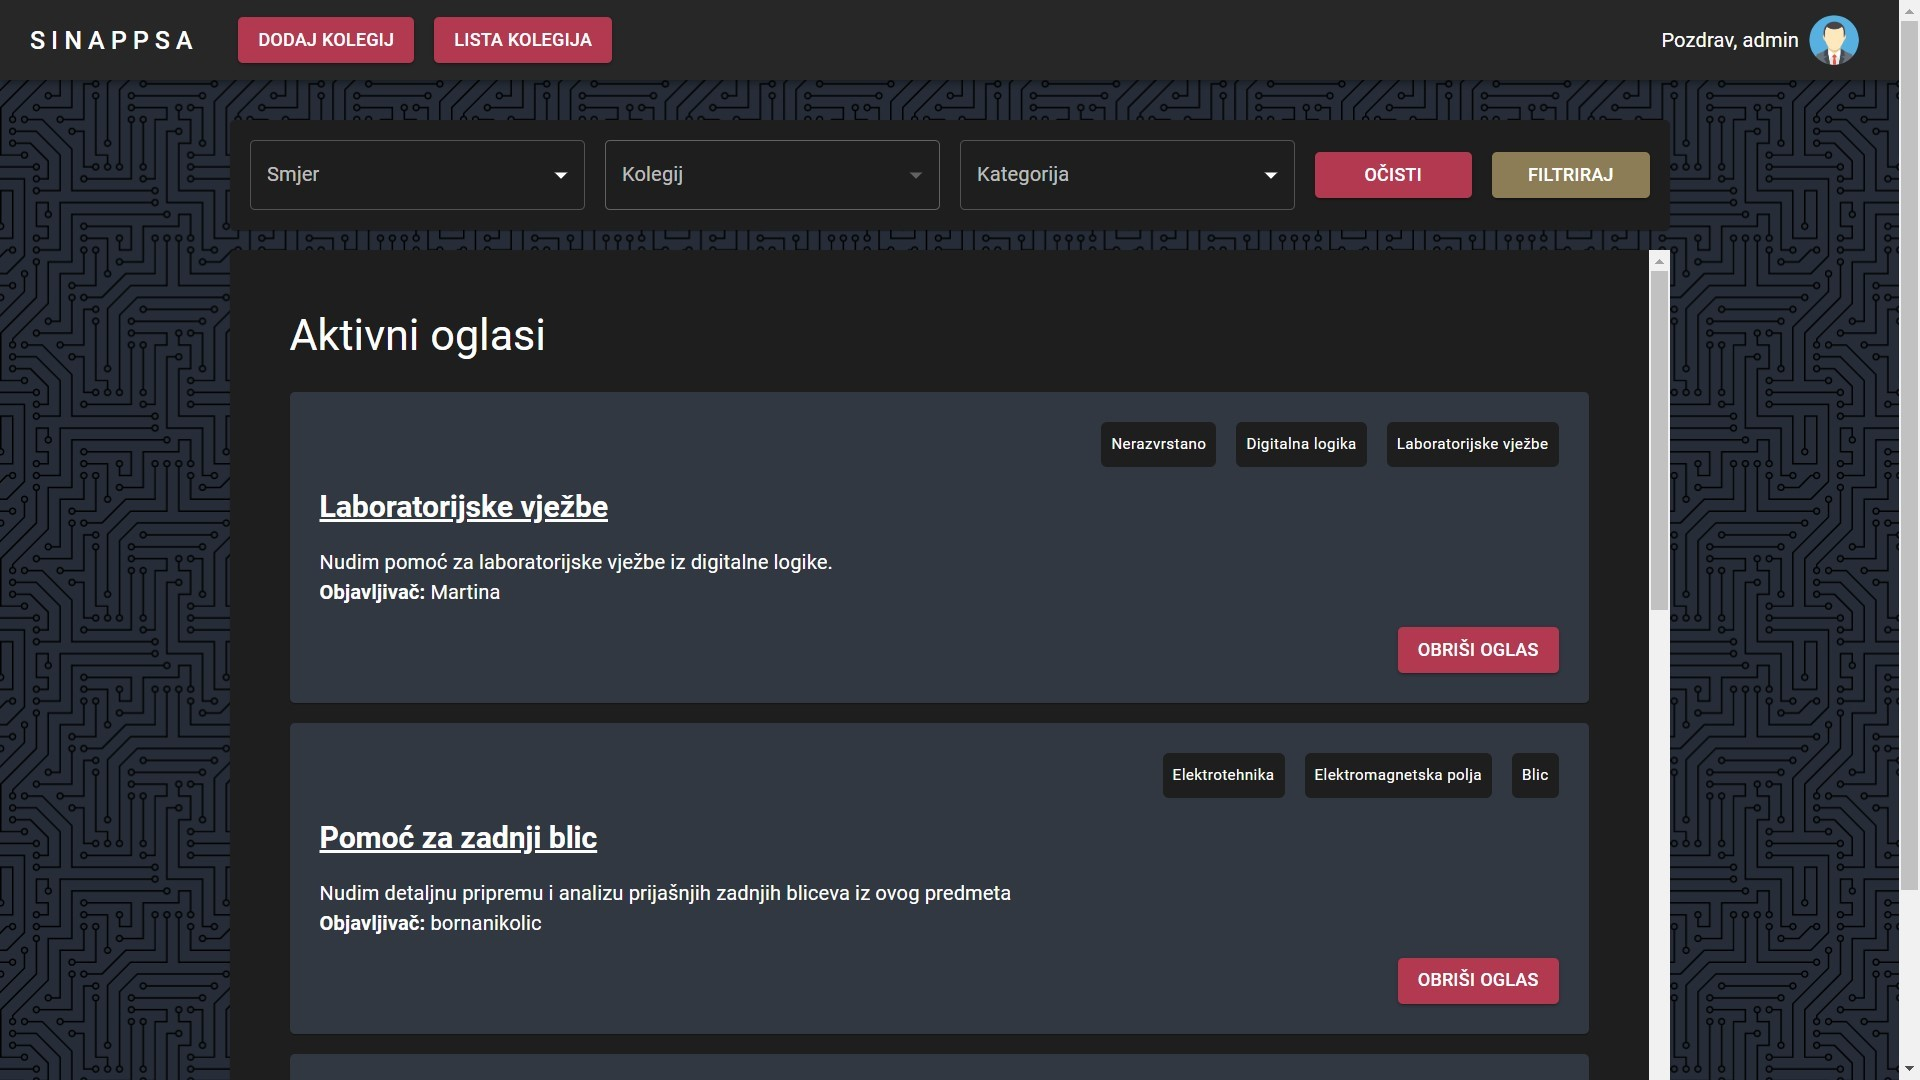
\includegraphics[scale=0.37]{slike/moderator1.jpg} 
				\centering
				\caption{Početna stranica za moderatora}
				\label{fig:moderator1}
			\end{figure}
		
			\begin{figure}[H]
				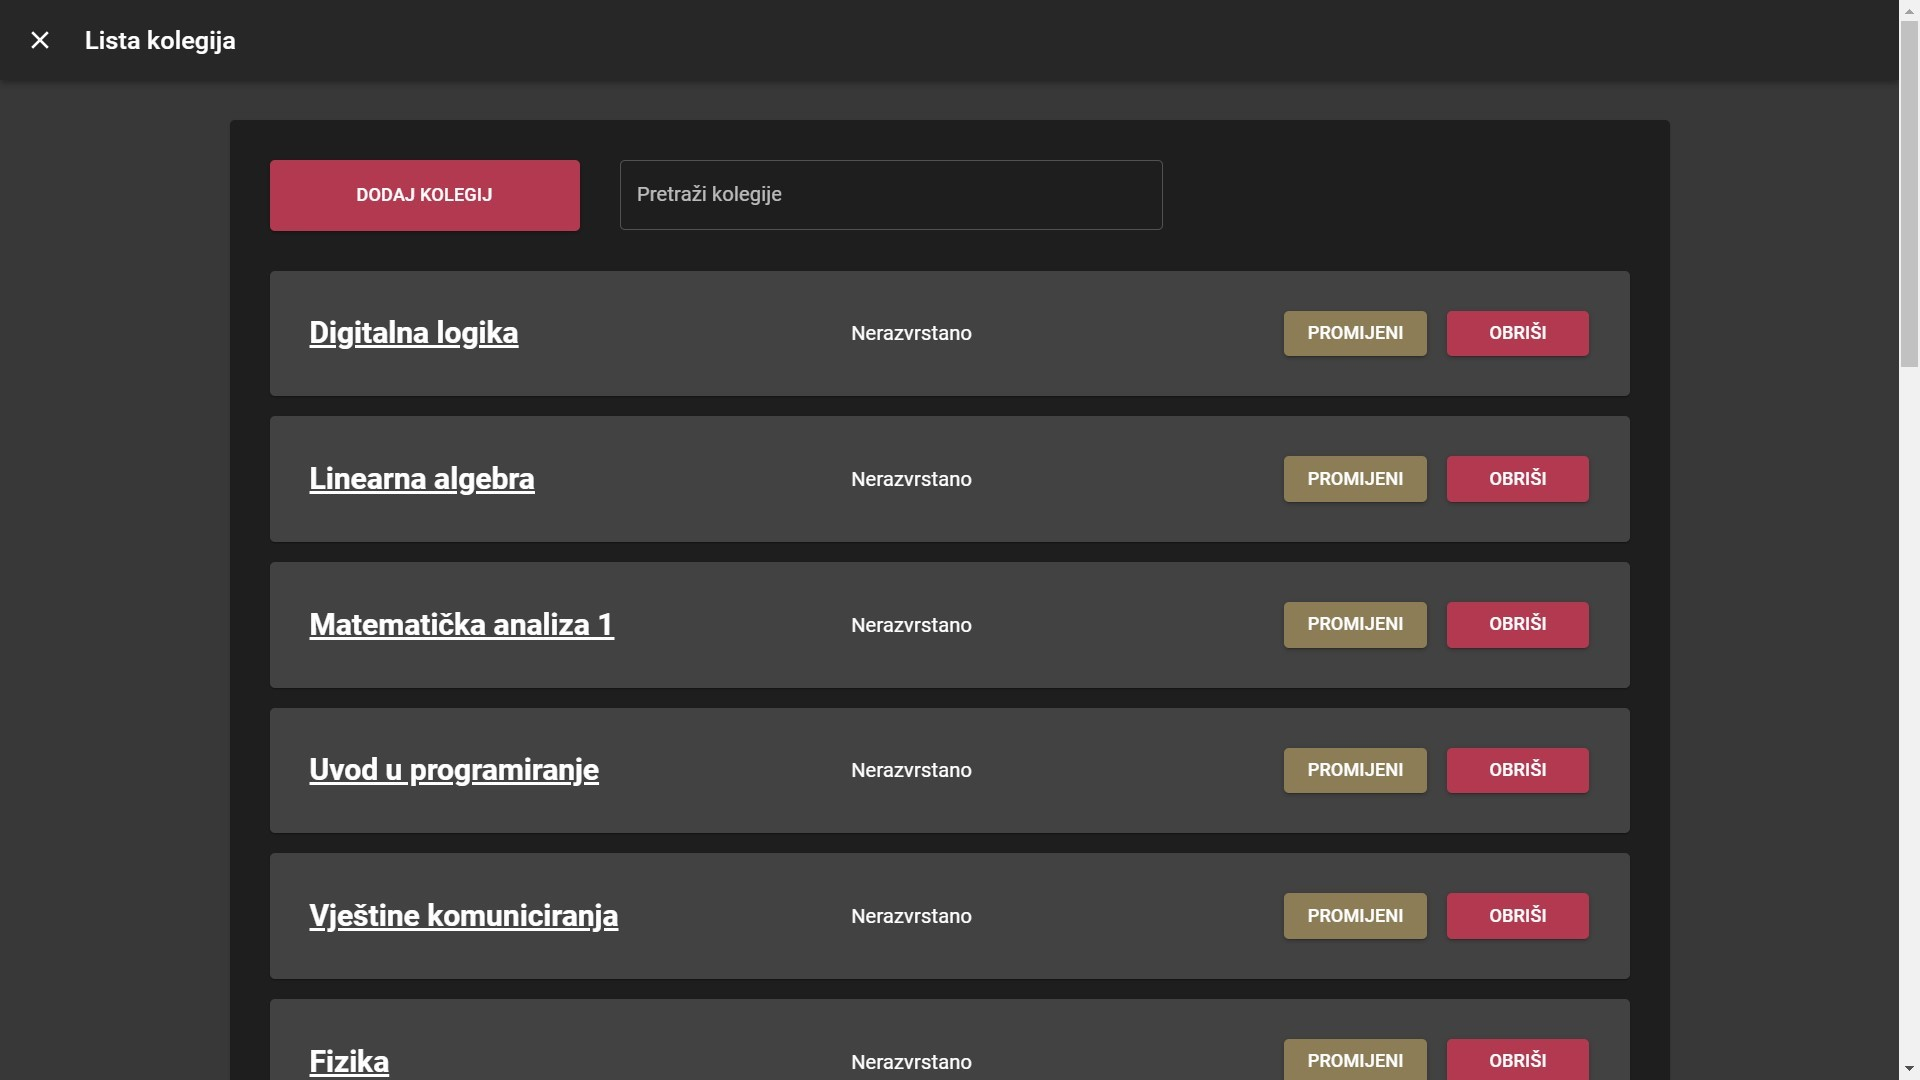
\includegraphics[scale=0.37]{slike/kolegiji.jpg} 
				\centering
				\caption{Lista dodanih kolegija}
				\label{fig:kolegiji}
			\end{figure}
		

		
		
	